\section{Exoplanets} \label{sect:exoplanets}
Since the first detection of an exo-solar planet around a main sequence star 
\parencite{mayor95}, 
the quest to find and study additional planets outside of our own solar system 
has been met with much enthusiasm and success. In recent years, numerous 
purpose-built instruments (e.g. \emph{HARPS}, 
%\cite{mayor03}, 
\emph{Kepler}, \& \emph{GPI}) 
%\cite{macintosh14} 
have been designed 
to detect these exoplanets using a variety of methods, each with their own 
unique advantages and biases. 
For instance, the radial velocity (RV) method, which uses stellar spectra to 
detect periodic Doppler 
shifts in spectral features thus indicating the presence of 
a companion, possibly planetary mass, is most sensitive to massive planets 
with short orbital periods.  \\

\emph{The results from many such dedicated exoplanet missions have been 
astounding.} Presently there are 2933 confirmed 
exoplanets\footnote{\url{http://exoplanets.org/}; accessed on June 28, 2016} 
with many thousands more planetary candidates. Furthermore, there 
exists a large diversity among planetary systems including the existence 
of certain exotic subsamples of exoplanets which do not contain an analog in 
our own solar system. Some of these extreme systems include i) the so-called hot 
Jupiters (e.g. 51 Pegasi b; \cite{mayor95}, HD 189733b; \cite{bouchy05}, 
\& HD 209458b; \cite{mazeh99, charbonneau00}); 
gas giant planets with masses comparable to or exceeding the mass of Jupiter, 
but with orbital periods of $\lesssim 20$ days, ii) circumbinary planets (e.g. 
Kepler-16b; \cite{doyle11}); 
planets which orbit stellar binaries, or iii) the most common type of 
planet in the local universe \parencite{petigura13}, 
namely super-Earths; planets with masses of 
$\sim 2-10$ M$_{\oplus}$ with a range of orbital separations (e.g. 
Gliese 581c,d; \cite{udry07} \& GJ 1214b; \cite{charbonneau09}).

\section{Methods of Detecting Exoplanets} \label{sect:detection}
I should probably talk about these a little bit but I don't think that it's 
important for the proposal. See Fig.~\ref{fig:detection}.
\begin{itemize}
\item Radial Velocity
\item Photometric Transit
\item Transit Timing/Duration Variation
\item Direct Imaging
\item Gravitational Microlensing
\item Astrometry
\end{itemize}

\begin{figure}
\centering
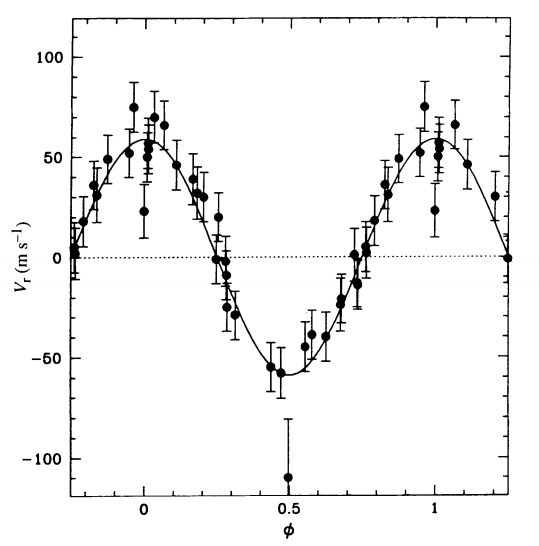
\includegraphics[scale=.2]{figures/51pegRV.png}
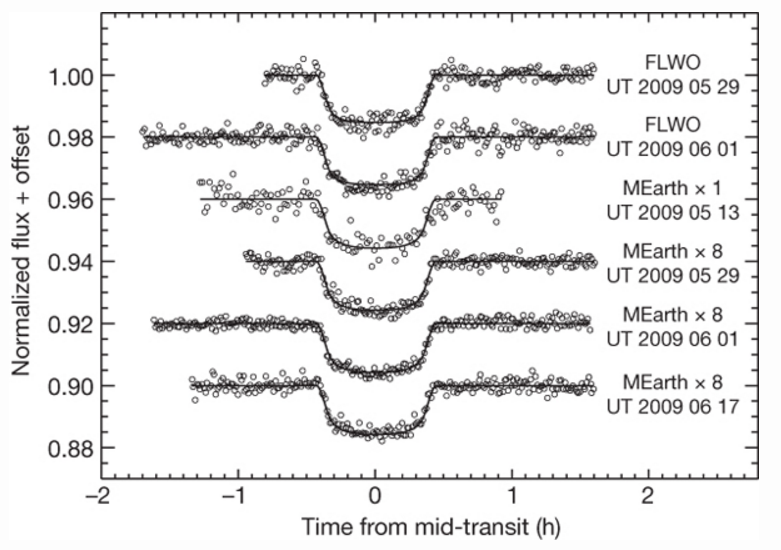
\includegraphics[scale=.2]{figures/gj1214transit.png}
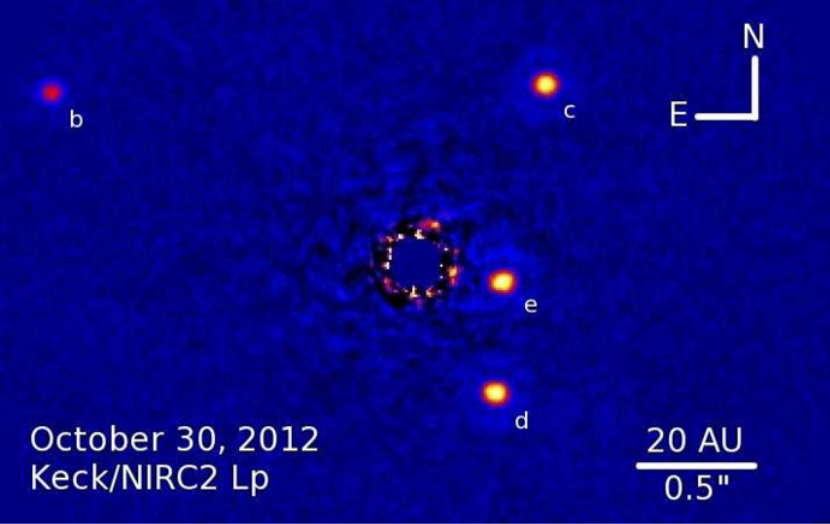
\includegraphics[scale=.2]{figures/hr8799nirc2.png}
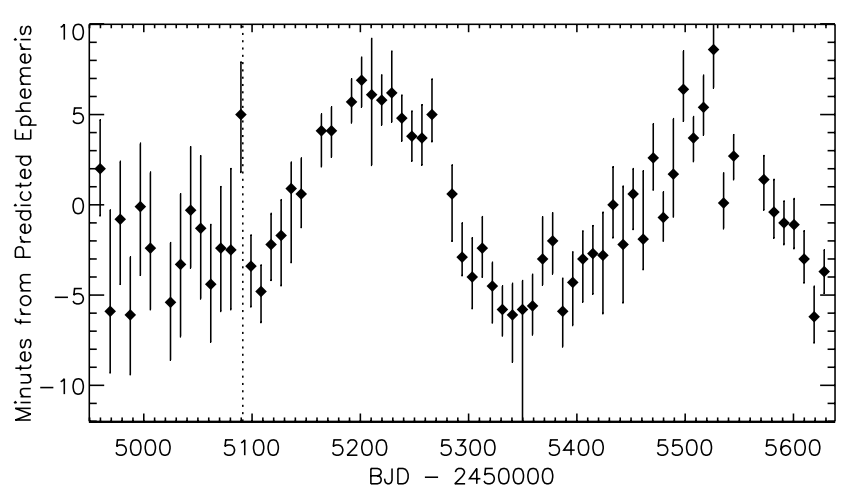
\includegraphics[scale=.22]{figures/kepler19bTTV.png}
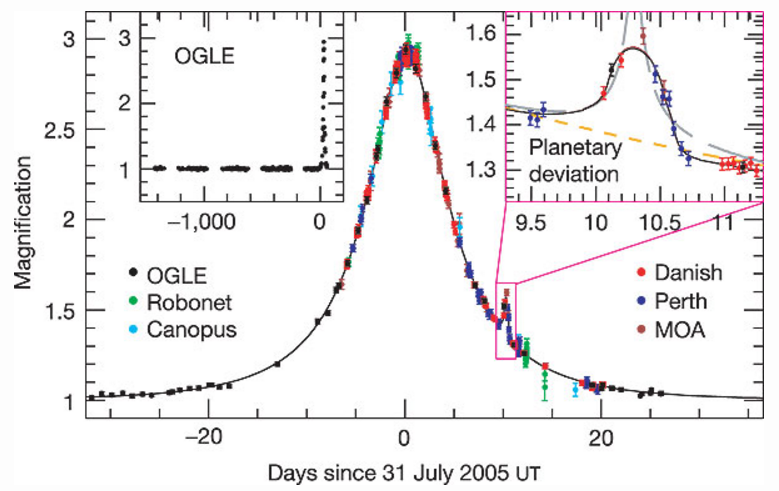
\includegraphics[scale=.2]{figures/ogle.png}
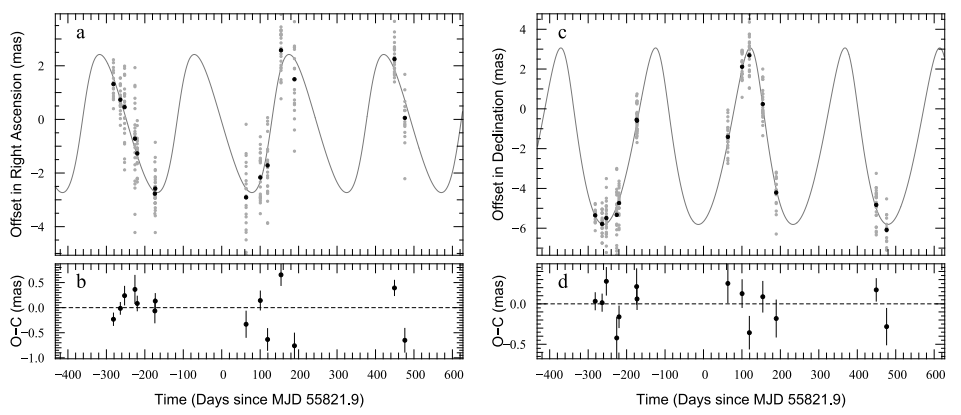
\includegraphics[scale=.24]{figures/de082349astrometry.png}
\caption{Examples of exoplanet detections with (\emph{clockwise from the 
top-left}) radial velocities \parencite{mayor95}, transits 
\parencite{charbonneau09}, TTVs \parencite{ballard11}, astrometry 
\parencite{sahlmann13}, gravitational microlensing \parencite{beaulieu06}, and 
direct imaging \parencite{currie14}. \label{fig:detection}}
\end{figure}

\section{Potentially Habitable Planets} \label{sect:HZ}
One highly sought after result arising from the endeavour of exoplanet hunting 
is the detection of potentially habitable Earth-like planets. 
Broadly speaking, a potentially habitable Earth-like planet refers to 
an exoplanet whose bulk composition is known to be rocky and whose 
orbital period places the planet within a range of distances from its host star 
where we expect water on the planetary surface to exist in its liquid phase; 
the habitable zone (HZ) \parencite{dole64, hart79}. Granted, this HZ 
definition is 
informed by our understanding of surface-based life on Earth and disregards 
the potential for additional, exotic forms of life such as water-based life 
in sub-surface oceans of planets. \\

Even with the limited definition of the 
HZ, it is known that numerous, and often unobservable factors complicate the 
exact definition of the HZ thus altering the expected orbital 
distances at which we should search for potentially habitable planets. 
Some of these factors include 

\begin{enumerate}
\item the presence of atmospheric greenhouse (GH) gases 
\parencite{kasting93, kopparapu13} which 
absorb thermal radiation from the planetary surface and re-emit roughly as a 
blackbody thus heating the planetary surface to temperatures exceeding the 
radiative equilibrium temperature expected in the absence of an atmosphere. 
\item The presence of clouds \parencite{selsis07, yang13} which increases the 
albedo thus causing the planet to be cooler than what is predicted by cloud-free 
models.
\item The planet mass \parencite{kopparapu14}. Assuming an atmospheric composition 
that is dominated by greenhouse gases (i.e. H$_2$O and/or CO$_2$) and that the 
amount of atmospheric volatiles scales with the planet mass, the surface pressure 
can be written in terms of the atmospheric column density $N$ and planet's 
surface gravity $g$ as 

\begin{equation}
\frac{P_{\mathrm{s}}}{P_{\mathrm{s}, \oplus}} = \left( \frac{N}{N_{\oplus}} \right)
\left( \frac{g}{g_{\oplus}} \right).
\end{equation}

\noindent Adopting an empirically derived mass-radius relation for planets with 
$m_p < 5$ M$_{\oplus}$, e.g. $m_p \propto r_p^{3.2}$ \parencite{kopparapu14}, 
the surface pressure increases with planetary mass as 

\begin{equation}
P_{\mathrm{s}} \propto m_p^{3/4}, 
\end{equation}

\noindent suggesting that more massive planets have thicker atmospheres.
\item Planetary rotation as the global atmospheric circulation dictates the 
spatial distribution of clouds. For instance, \parencite{yang14} showed that 
slowly rotating planets can maintain hospitable climates over longer timescales than 
rapid rotators.
\item Relevant system geometries such as planet obliquity 
\parencite{williams97, spiegel08, spiegel09} and orbital eccentricity 
\parencite{dressing10, cowan12}. 
\end{enumerate}

This list of effects on planetary habitability represents a subset of the 
seemingly infinite (\textbf{exaggeration}) number of factors which determine 
whether or not an Earth-like biosphere can exist on an exo-solar planet. 
Luckily each of these properties can in principle be measured, at least for 
a subset of planets which are conducive to such observations. For example, 
for factors 1,2) above, 
the presence of particular chemical species and clouds/hazes 
in a exoplanetary atmosphere 
can be detected via variations in the apparent size of the planet as a function 
of wavelength; transmission spectroscopy \parencite{seager00}, 3) the planet 
mass can be measured from radial velocities and/or transit timing variations 
\parencite{holman05}, 4) the planetary rotation rate can be measured if the 
planetary spectrum can be distinguished from that of its host star and if the 
rotation rate is sufficiently large such that the rotational line broadening 
is detectable \parencite[e.g.][]{snellen14, schwarz16}, and 5) the planetary obliquity or 
spin--orbit misalignment can be measured for transiting planets using 
spectroscopy \parencite{rossiter24, mclaughlin24, queloz00} and their orbital 
eccentricities measured from radial velocities or secondary eclipse observations of 
transiting planets. \\

To date, a number of potentially habitable, Earth-like candidates have already 
been detected \parencite[e.g. Kepler-438b, 442b;][]{torres15}). Although, these 
inferences of habitability are based on a limited number of arguments for the 
planet's size, mass,\footnote{Therefore its bulk density 
($\rho \propto m_p/r_p^3$) and surface gravity ($g \propto m_p/r_p^2$).} and 
insolation relative to Earth. Knowledge regarding the atmospheres and surface 
conditions of these planets still remains largely uncertain. Fortunately, 
atmospheric 
characterization is possible through techniques such as transmission and/or 
emission spectroscopy of transiting planets and near edge-on planets 
respectively. These methods have been successfully performed for a small 
sample of \emph{non-rocky} exoplanets only 
\parencite[e.g.][]{bean13, crouzet14, kreidberg14, mccullough14}. 

\subsection{Adopted HZ Definition}
We opt to restrict our focus of HZ planets to the commonly used definition 
\parencite{kasting93} and parametric model of \cite{kopparapu13}. 
In this definition the inner edge of the HZ 
is defined by the `moist GH' or `water-loss' limit wherein a slight increase 
in flux results in the 
photodissociation of water vapour and subsequent hydrogen escape in the upper 
atmosphere. The outer edge is then given by the `maximum GH' wherein any 
addition of CO$_2$ into the atmosphere results in a net cooling effect as the 
increased Rayleigh scattering (increased albedo) begins to dominate over the 
added GH effect resulting in a net cooling. \\

The parametric model \parencite{kopparapu13} relates the orbital separations 
$a$ of the inner and outer edges of the HZ to the insolation received by planets 
at those distances. To compute the HZ edges for a given star requires its 
luminosity $L$ and effective temperature $T_{\mathrm{eff}}$ 
as input parameters. Specifically,

\begin{equation}
a = 1 \mathrm{\hspace{2pt} AU} \cdot \sqrt{\frac{L/L_{\odot}}{S_{\mathrm{eff}}}},
\end{equation}

\noindent where

\begin{equation}
S_{\mathrm{eff}} = S_{\mathrm{eff},\odot} + AT_* + BT_*^2 + CT_*^3 + DT_*^4,
\end{equation}

\noindent where $T_* \equiv T_{\mathrm{eff}}-5780$ K and the coefficients 
$S_{\mathrm{eff},\odot},A,B,C,D$ are computed for the `moist-GH' and `maximum-GH' 
limits (reported in \cite{kopparapu13}). This model is applicable to all 
early-to-mid M-dwarfs and down to ultracool dwarfs with $T_{\mathrm{eff}}$ as 
low as 2600 K. \\

Finally we relate the orbital separations of the HZ edges to the observable 
orbital period $P$ using Kepler's third law:

\begin{equation}
P^2 \sim \frac{4 \pi^2}{G M_s} a^3.
\label{eq:keplersthird}
\end{equation}


\iffalse
Atmospheric transmission and emission spectroscopic techniques require 
bright host stars in order to acquire high signal-to-noise observations and is 
therefore naturally favoured by nearby targets. Therefore, to obtain  
atmospheric characterization of a rocky world with powerful upcoming 
instrumentation \citep[e.g. \emph{NIRISS} aboard \emph{JWST};][]{doyon12} we 
must first detect this population of nearby rocky exoplanets. To date, the 
highest priority terrestrial planet for atmospheric characterization is 
GJ 1132b \citep{berta15} at just 12 pc. Using the occurrence rates of small 
planets around M-dwarfs from \cite{dressing15a}, they estimated that the 
nearest 
\emph{transiting} potentially habitable rocky planet is within 14.6 pc at 95\% 
confidence. GJ 1132b may therefore represent this planet. Integrating over 
planetary system inclinations, \cite{dressing15a} estimated that the nearest 
potentially habitable rocky planet is within just 3.5 pc at 95\% confidence. 
We have yet to discover such a planet but radial velocity efforts are 
currently being built and tested 
\citep[e.g. \spirou{;}][]{thibault12, artigau14} to achieve precisely this 
goal; finding the closest potentially habitable world. 
\fi

\section{Exoplanet detection via Stellar Radial Velocity} \label{sect:RV}
\subsection{Radial velocity curves}
The radial velocity (RV) method of detecting exoplanets represents a simple 
application of Newton's third law: `for every action, there is an equal 
and opposite reaction'. In our case, the presence of planetary companions to a 
host star displaces the centre-of-mass of the system from the centre of the star 
itself. Because of this, a star with a single companions 
executes an orbit about the system's centre-of-mass 
with an approximate velocity 

\begin{equation}
v(t) = V_0 + K[\cos{(\nu(t,P,\mathrm{T}0) + \omega)} + e\cos{\omega})],
\label{eq:rv}
\end{equation}

\noindent where $V_0$ is the systemic velocity offset, 
$t$ is the independent time coordinate, $P$ is the orbital period of the star/planet, 
T0 is the reference epoch or time of mid-transit\footnote{More generally, T0 is the 
epoch at which the planet is closest to the observer in its orbit.}, 
and $K$ is the semi-amplitude of the velocity variation 
which is dependent on system body masses and orbit 
(see Sect.~\ref{sect:K}). Eq.~\ref{eq:rv} is known as the keplarian orbital 
solution. The orbital elements $e$ and $\omega$ are the orbital 
eccentricity and argument of periastron respectively. Note that $\omega$ is only 
defined for non-zero eccentricities. 
The true anomaly $\nu(t)$ then defines the position of the star on its orbit 
relative to the argument of periastron in the direction of motion and is derived 
from another angular parameter, namely the eccentric anomaly $E$. The eccentric 
anomaly $E$ can be solved for using the mean anomaly $M$ according to 
Kepler's equation

\begin{equation}
M(t) = E(t)-e\sin{E(t)},
\label{eq:kepler} 
\end{equation}

\noindent where the mean anomaly is

\begin{equation}
M(t) = \frac{2\pi}{P} (t-\tau_{\mathrm{peri}}), 
\end{equation}

\noindent and $P$ is the orbital period and $\tau_{\mathrm{peri}}$ is the time of 
pericenter passage. Because Eq.~\ref{eq:kepler} does not have a closed-form 
solution, it must be solved using iterative numerical techniques. 
Examples of keplarian orbits from Eq.~\ref{eq:rv} are shown in Fig.~\ref{fig:rv} 
for two 
Earth-mass planets each with an orbital period of 10 days around a 0.1 M$_{\odot}$ 
M-dwarf. The first planet is on a perfectly circular orbit and therefore 
has a purely sinusoidal 
velocity while the second planet's eccentricity is 0.5 and whose velocity 
clearly differs from purely sinusoidal with the addition of the second 
cosine term in Eq.~\ref{eq:rv}. \\

\begin{figure}
\centering
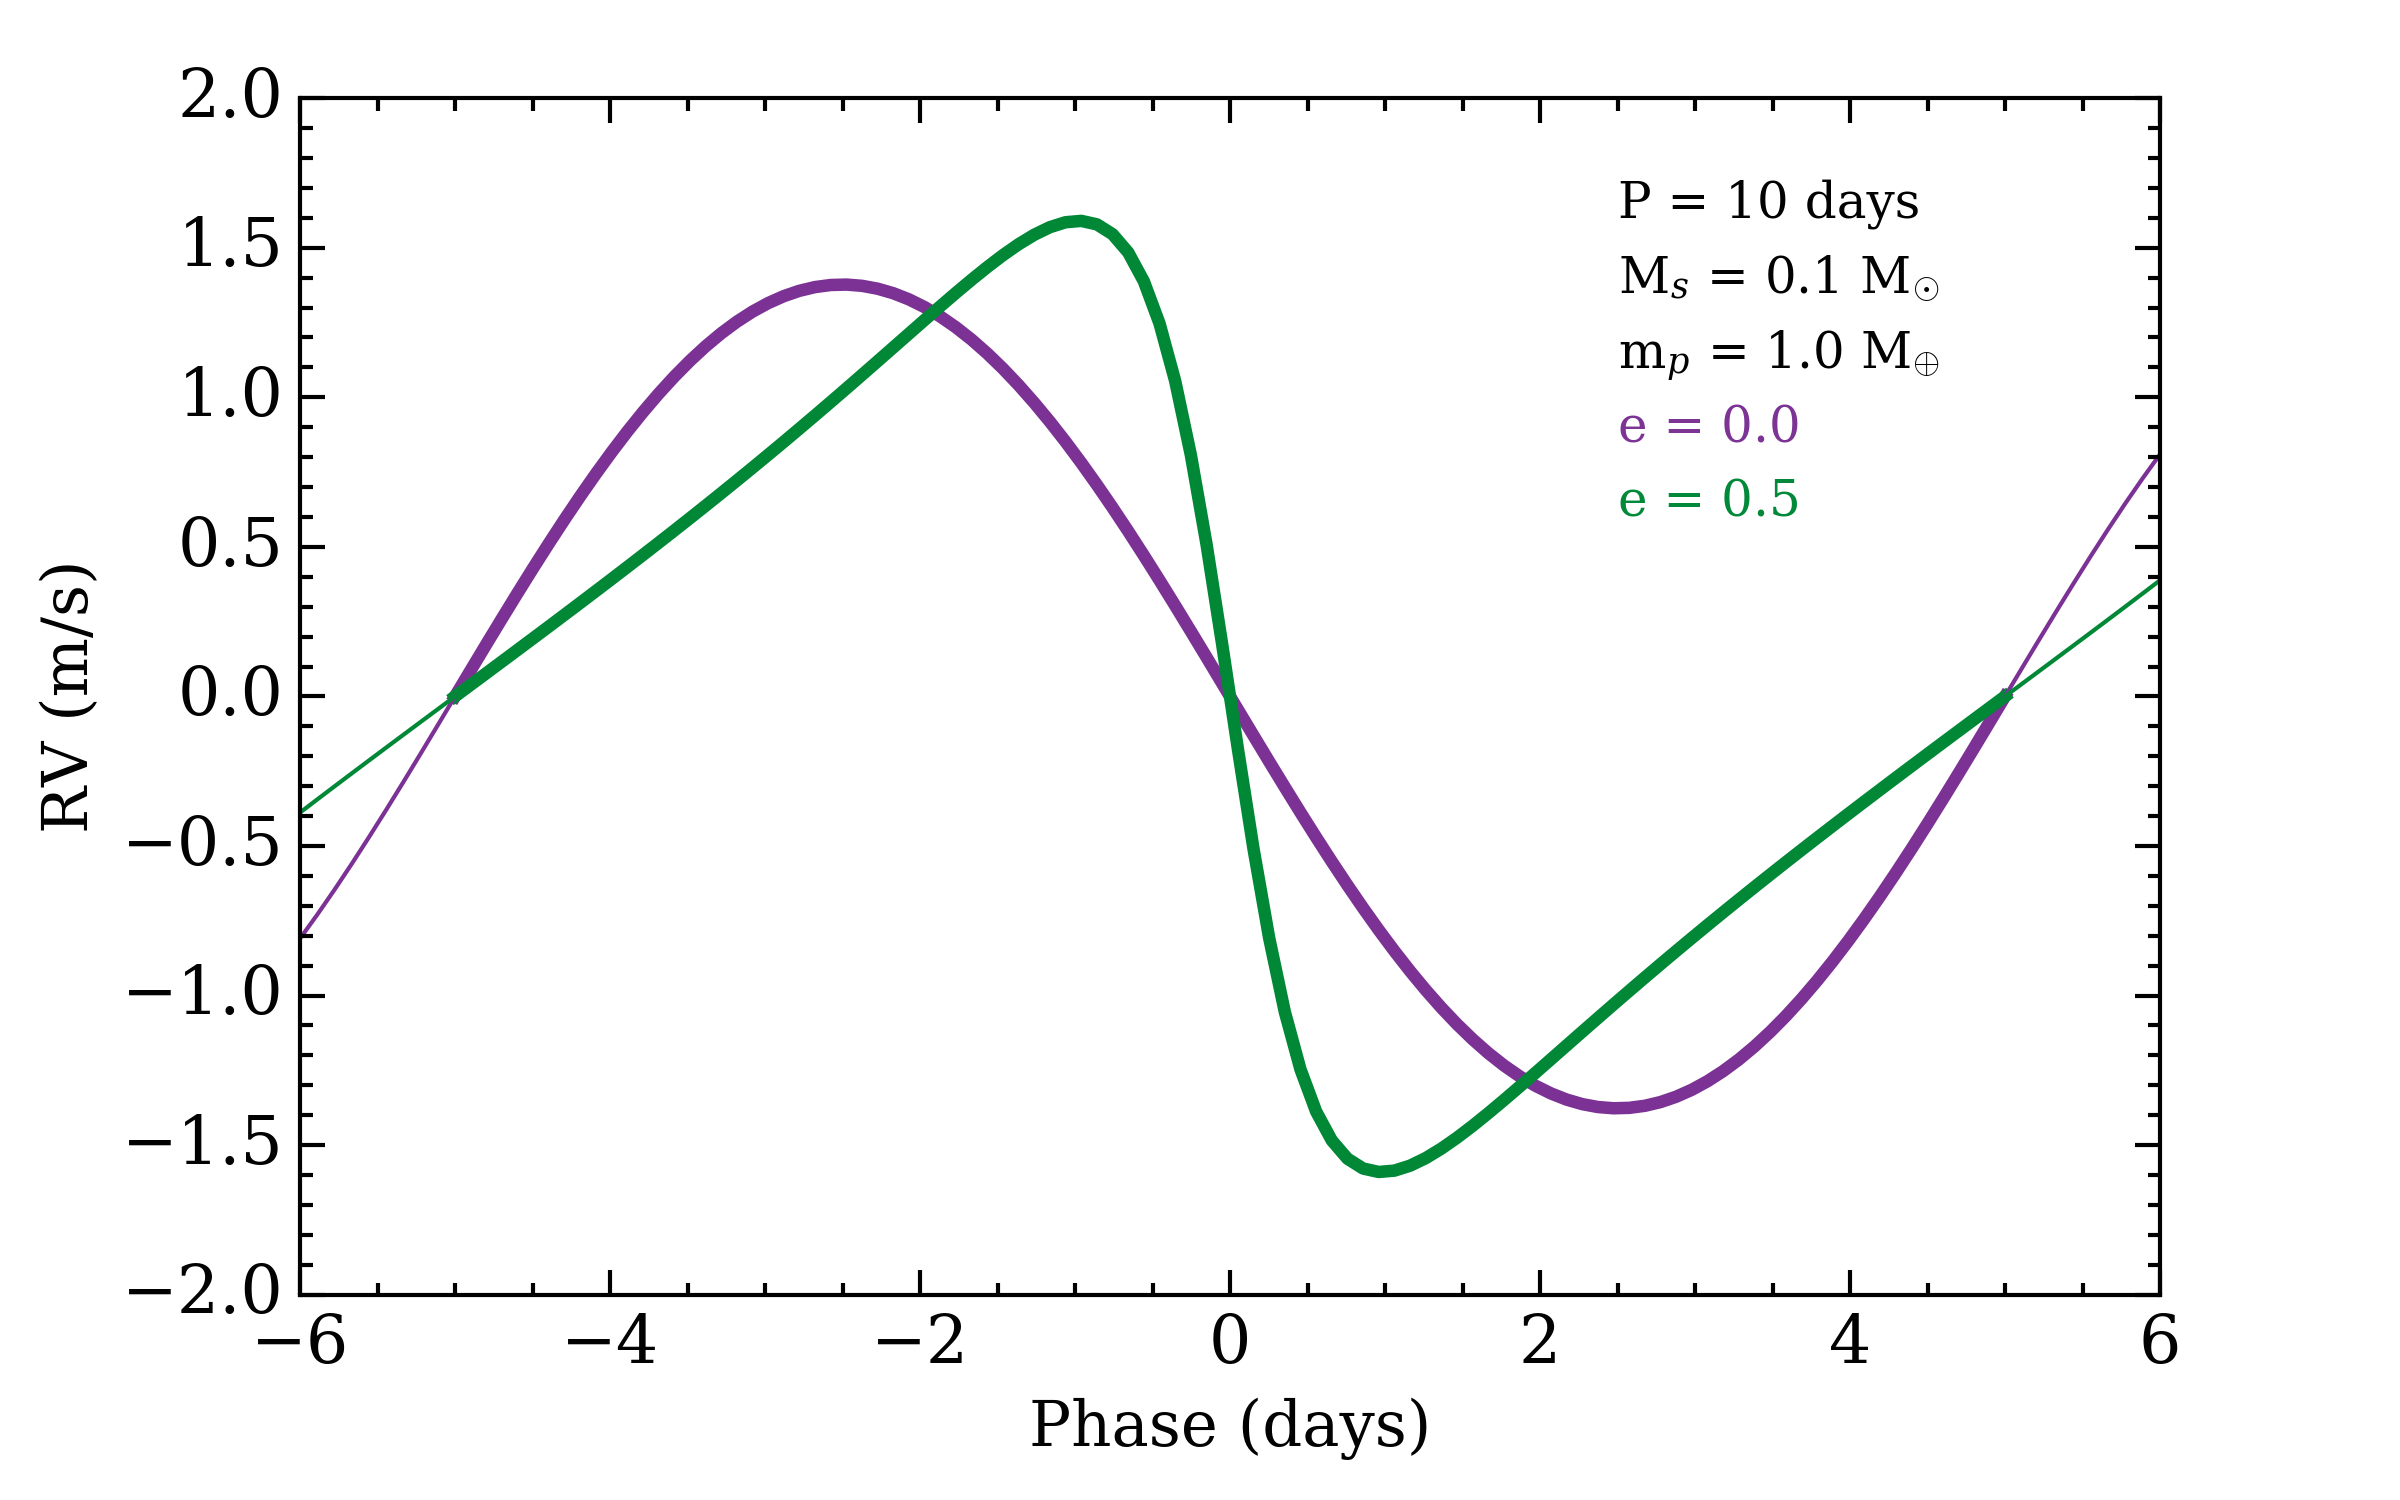
\includegraphics[scale=0.6]{figures/rvcurve_example.png}
\caption{Keplarian orbital solutions for two planets each with an orbital period of 10 days 
and one Earth mass orbiting a 0.1 M$_{\odot}$ star. The \emph{blue} planet is on a 
perfectly circular orbit ($e=0$) while the \emph{green} planet's orbit has a significant 
eccentricity ($e=0.5$). Note the deviation of the latter from a pure sinusoid. \label{fig:rv}}
\end{figure}

The keplarian orbital solution is valid in the absence of dynamical 
perturbations to the 2-body system. In this case only the true anomaly varies with 
time. However if additional bodies are present in the system such as in binary star 
systems or in compact high multiplicity planetary systems, then the parameters in 
Eq.~\ref{eq:rv} need not be fixed and we instead refer to the measured orbit as the 
osculating orbit which may vary between orbital cycles. Note that if the timescale 
for perturbations to the stellar orbital solution is comparable to or less than the 
time interval over which radial velocity observations are taken, then the keplarian 
orbital solution is insufficient and one must consider a more complicated treatment 
of the dynamics typically in the form of N-body simulations.

\subsection{Measurements from the radial velocity method} \label{sect:K}
If we consider the simplest planetary system, we have a star and planet each 
orbiting their common centre-of-mass (COM) with position vector

\begin{equation}
\mathbf{r}_{\mathrm{COM}} = \frac{M_s \mathbf{r}_s + m_p \mathbf{r}_p}{M_s + m_p}.
\end{equation}

\noindent To simplify the configuration further let us assume that the star is 
much more massive than its planetary companion ($M_s \gg m_p$) and that the 
COM coordinate is located at the origin ($|\mathbf{r}_{\mathrm{COM}}|=0$). Working 
in absolute scalar terms, the orbital distances of the star and planet are then 
related via 

\begin{equation}
a_s = a \left( \frac{m_p}{M_s} \right)
\label{eq:com}
\end{equation}
  
\noindent where we have changed notation by writing $|\mathbf{r}_s|$ as $a_s$ and 
$|\mathbf{r}_p|$ as $a$. For a perfectly circular orbit ($e=0$), the constant 
velocity of the star around the COM is 

\begin{equation}
v = \frac{2\pi a_s}{P}.
\label{eq:velocity}
\end{equation}

\noindent As the star orbits the COM as a result of the gravitational influence its 
planetary companion, the maximum observed radial velocity of the star is realized 
when the radial component of the star's 3D 
velocity is maximized. At these points in the orbit $v$ equals the semi-amplitude 
of the radial velocity curve $K$. Because the radial velocity 
curve and hence $K$, is observable, 
we can relate $K$ to the masses of the star and planet by combining the velocity 
equation (Eq.~\ref{eq:velocity}) with Kepler's third law and the COM equation 
(Eqs.~\ref{eq:keplersthird} \& \ref{eq:com} respectively):

\begin{align}
\mathrm{max}(v(t)) = K &= \frac{2\pi a_s}{P}, \\
&= \frac{2\pi}{P} \left( \frac{m_p}{M_s} \right) a, \\
&= \frac{2\pi}{P} \left( \frac{m_p}{M_s} \right) \left( \frac{GM_s}{4\pi^2} \right)^{1/3} P^{2/3}, \\
&= \left( \frac{2\pi G}{M_s^2 P} \right)^{1/3} m_p. \label{eq:K1}
\end{align}

Eq.~\ref{eq:K1} contains two observables directly from the RV timeseries: the orbital 
period $P$ and semi-amplitude $K$. Typically an observer will use the stellar spectra 
from which the radial velocity measurements are computed, in tandem with spectral 
templates to infer the spectral type and stellar mass of the host star. This allows 
us to infer the mass of the planetary companion from the RV timeseries. The uncertainties 
in the planet mass 
measurement are typically dominated by the noise in dataset and uncertainties in 
the best-fit stellar mass from spectral fitting. \\

Looking more closely at Eq.~\ref{eq:K1} we can see that the RV semi-amplitude scales 
linearly with planet mass but has a negative scaling with stellar mass and orbital 
period. This makes sense because the radial velocity effect is gravitational in 
nature. A larger perturbing mass ($m_p$) will result in a larger perturbation to the 
central body which itself becomes more difficult to perturb if more massive. Also the 
effect weakens when the distance between the bodies is increased (larger $P$). The 
radial velocity method therefore has a natural observational bias towards massive, 
close-in planets around small stars. This explains why the first planets to be 
detected with the radial velocity method were hot Jupiters 
\parencite[e.g.][]{mayor95}. For reference, the RV semi-amplitude that the Earth 
induces on the Sun is $\sim 9$ cm s$^{-1}$ whereas the more massive Jupiter induces a 
$\sim 12$ \mps{} effect despite having a much wider orbit.

\subsection{Caveats to Eq.~\ref{eq:K1}}
In the derivation of the RV semi-amplitude (Eq.~\ref{eq:K1}) we have neglected two 
important geometric effects. The first is that of eccentricity which, if non-zero, 
causes the stellar radial velocity to vary throughout the orbit; $K \ne v$. Instead 
$K = \mathrm{max}(v(t))$ and increases because the conservation of angular momentum 
requires that $v(\tau_{\mathrm{peri}})$ 
be greater than elsewhere on the orbit. The corresponding correction 
factor to Eq.~\ref{eq:K1} is $(1-e^2)^{-1/2}$. \\

The second effect is that of inclination. When attempting to measure the planetary 
mass from radial velocities the orbital inclination of the planetary orbit\footnote{Orbital 
inclination is conventionally measured  relative 
to the plane of the sky; i.e. an edge-on orbit has $i=90^{\circ}$.} is entirely unknown 
unless the planet has a well-defined transit model which is sensitive to the orbital 
inclination. But for the majority of planets which are not transiting, the orbital inclination 
is unknown and degenerate with $m_p$. Therefore for most planets, radial velocity measurements 
are only sensitive to a mass lower limit $m_p\sin{i}$ rather than the absolute planet mass. \\

Compared to Eq.~\ref{eq:K1}, 
a more complete description of the RV semi-amplitude is therefore 

\begin{equation}
K = \left( \frac{2\pi G}{M_s^2 P} \right)^{1/3} \frac{m_p \sin{i}}{\sqrt{1-e^2}}. 
\label{eq:K2}
\end{equation}

\section{Measuring Radial Velocities} \label{sect:spectrograph}
Radial velocity variations induced by planetary companions cause the star to become 
periodically Doppler shifted. These wavelength shifts can be detected using hi-resolution 
spectroscopy as absorption features in the stellar photosphere are shifted from their 
rest wavelength $\lambda_{\mathrm{rest}}$ as the star's velocity changes along the line-of-sight 
according to 

\begin{equation}
\frac{\Delta \lambda}{\lambda_{\mathrm{rest}}} = \frac{v}{c}.
\end{equation}

\noindent In practise, the velocity shift is measured from the cross-correlation function of 
the observed stellar spectrum with a template spectrum of the same spectral type. The highest 
precision is achieved when the results from many lines can be averaged. This makes the radial 
velocity method rather tractable for M-dwarfs in particular which exhibit a plethora of 
spectral lines, particularly oxide molecular lines including titanium oxide (TiO) and vandium 
oxide (VO) for ultracool dwarfs. A sample of infrared spectra of early-to-late M-dwarfs 
are shown in Fig.~\ref{fig:spectra} to demonstrate the wealth of absorption features. 
These spectra from \cite{rayner09} were obtained 
with SpeX at NASA's Infrared Telescope Facility at a resolving power of 
$R=\lambda / \Delta \lambda \sim 2000$. \\ 

\begin{figure}
\centering
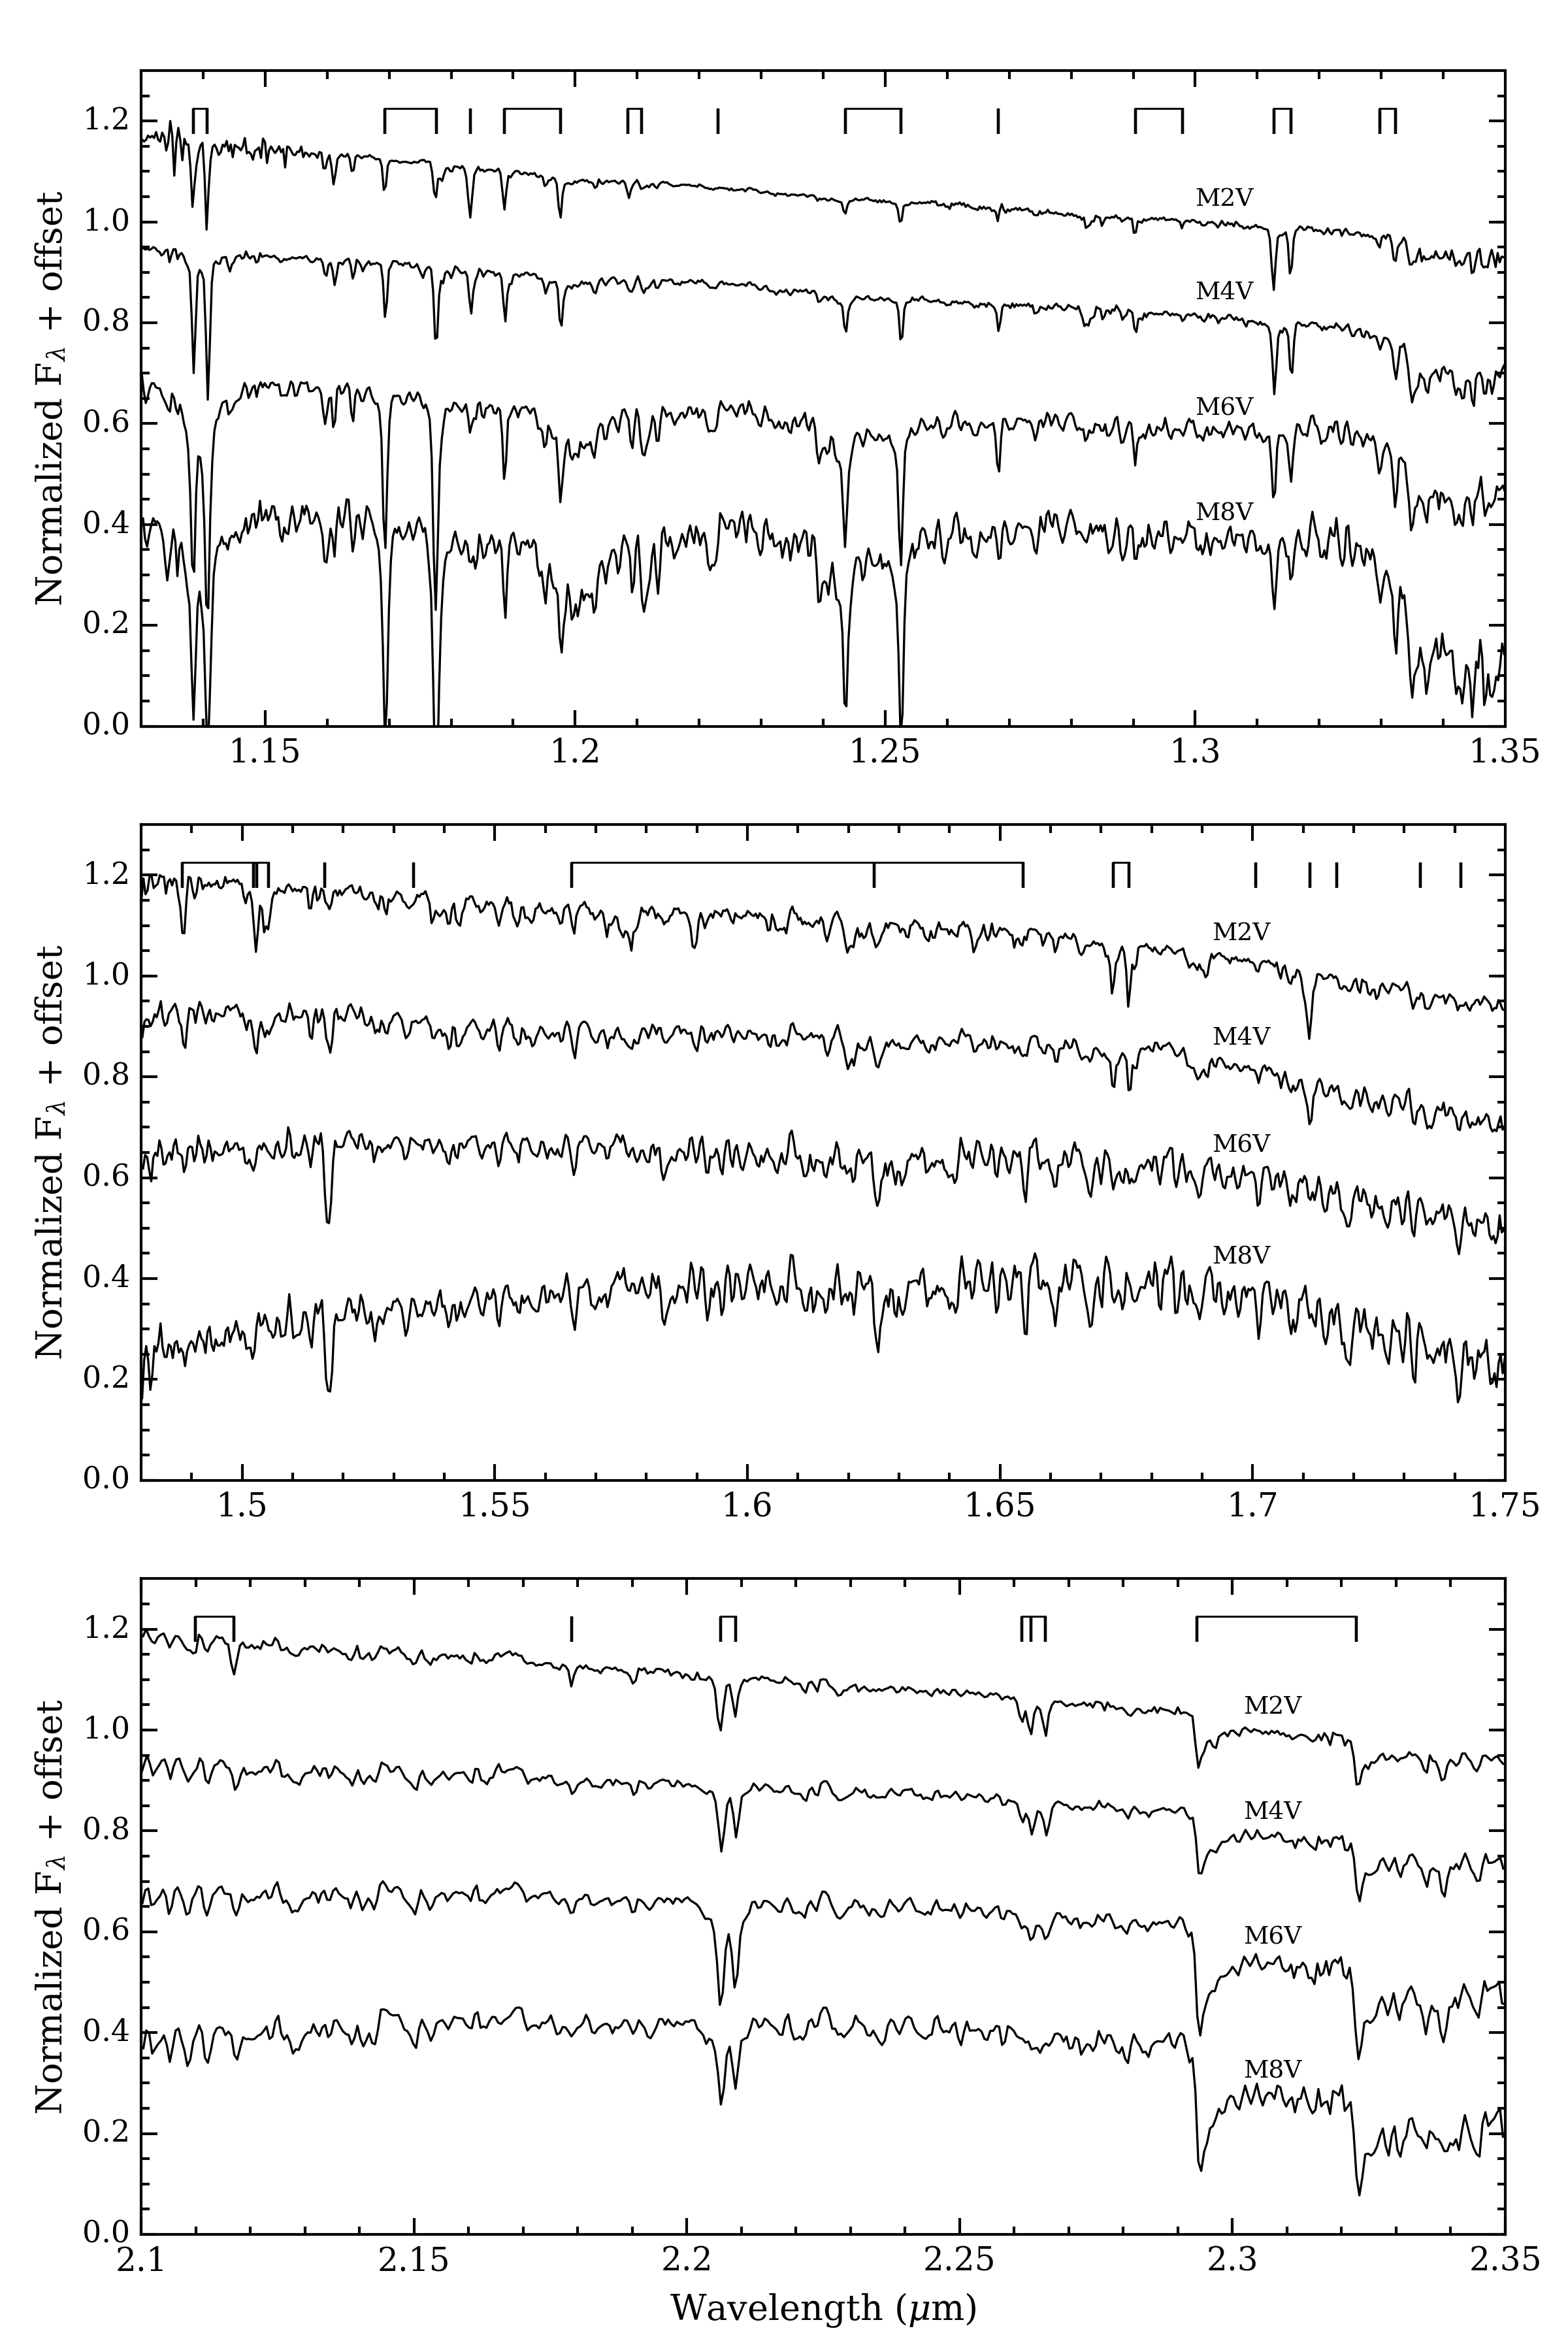
\includegraphics[scale=0.7]{figures/Mdwarf_spectra.png}
\caption{Infrared spectra of four M-dwarfs in the J band (\emph{top}), H band 
(\emph{middle}), and K band (\emph{bottom}). \label{fig:spectra}}
\end{figure}

The spectroscopic measurements are made with a spectrograph containing a grating which 
diffracts the incoming source light into spectral orders which are subsequently 
cross-dispersed spatially. The dispersed spectral orders are projected onto a detector 
to create the observed stellar spectrum. The spectrum is then cross-correlated with a  
template rest frame spectrum from the lab. The cross-correlation of prominent lines 
are averaged to create the cross-correlation function (CCF) of the star at the epoch of 
observation. The CCF is typically fit with a Gaussian line profile whose best-fit mean 
is equal to the measured radial velocity \parencite{pepe02}. 
Active regions on the stellar surface arising 
from the presence of magnetic fields can have additional effects on the observed CCF 
causing the line profile to be exhibit non-Gaussianities. 
As we shall see in Sects.~\ref{sect:fwhm} and \ref{sect:bis}, these distortions can 
be used to model the stellar activity which can then be subtracted to possibly reveal 
any present planetary signals in radial velocity.

\section{Point-form Thesis: Introduction}
\begin{itemize}
\renewcommand\labelitemi{--}
\item~\ref{sect:exoplanets} \textbf{Exoplanets}: in the local universe exoplanets are 
extremely abundant and quite diverse compared to the planets in our own solar system.
\item~\ref{sect:detection} \textbf{Methods of Detecting Exoplanets}: there exists a 
number of methods of detecting exoplanets each with their own sensitivity to particular 
planetary systems.
\item~\ref{sect:HZ} \textbf{Potentially Habitable Planets}: rocky planets which lie in 
their host star's nominal habitable zone are interesting targets which are flagged as 
potentially habitable. The habitable zone is defined by planetary surface temperatures 
where liquid water can be sustained.  
\item~\ref{sect:RV} \textbf{Exoplanet Detection via Stellar Radial Velocity}: the 
periodic gravitational influence of planetary companions on their host star can be 
detected thus measuring a lower limit on the planetary mass and the planet's orbit.
\item~\ref{sect:spectrograph} \textbf{Measuring Radial Velocities}: hi-resolution 
spectrographs are used to measure the Doppler shift of stellar absorption features; 
the star's radial velocity.
\end{itemize}
